% -*-coding: utf-8 -*-
% Держать в начале каждого файла!

\documentclass[a4paper, 12pt]{extarticle}
% 14 пт - жесть
\usepackage{metod}

\MTDSetPhysSection{Механика}
\MTDSetTitle{Введение в теорию погрешностей. Измерения в физическом практикуме}
\MTDDesignator{М--0}
\MTDSetGrade{10}

\MTDSetAuthors{И.~Н.~Грачева, В.~И.~Гребенкин, А.~Е.~Иванов, И.~А.~Коротова,
Е.~И.~Красавина, А.~В.~Кравцов, Н.~С.~Кулеба, Б.~В.~Падалкин,
Г.~Ю.~Шевцова, Т.~С.~Цвецинская}

\MTDSetEditorsGenCase{И.~Н.~Грачевой, А.~Е.~Иванова, А.~В.~Кравцова}

\newcommand{\eps}{\epsilon}
\newcommand{\nisum}{\sum\limits_{i=1}^{i=n}} %WTF?!
\newcommand{\isum}{\sum\limits_{i=1}^{n}}

\begin{document}

\MTDTitlePage
\MTDInfoPage

% В начале каждой лабы надо задать номер секции, чтобы правильно работали

% Мелкий хак - если
\section*{Предисловие}
Физический практикум содержит описания лабораторных работ для учащихся 10-х классов лицея \textnumero1580 при МГТУ имени Н.~Э.~Баумана.

На выполнение каждой работы отводится два академических часа занятий. Подготовку к выполнению работ учащиеся производят в часы их самостоятельной работы.

Основной задачей лабораторных занятий является приобретение навыков в обращении с измерительными приборами, знакомство с простейшими приемами обработки результатов измерений и привитие учащимся навыков самостоятельной работы.

Наряду с этим выполнение лабораторных работ способствует более осознанному пониманию физических явлений и законов.

В описании работ даны краткая теория, методика выполнения работы, последовательность измерительных операций, а также простейшие приемы обработки результатов измерений.

\section*{Методические указания}
При подготовке к выполнению лабораторной работы нужно ознакомиться с ее содержанием, изучить по рекомендованной литературе теоретический материал, дать ответы на контрольные вопросы, продумать измерительные операции, оформить лабораторный журнал. В качестве лабораторного журнала используют общую тетрадь. Оформление каждой работы начинают с новой страницы.

В тетрадь вписывают название, номер работы, дату выполнения, цель, схемы установки, перечень приборов, таблицы, расчетные формулы.

Для вспомогательных записей и расчетов отводят четные страницы; схемы, таблицы выполняются в карандаше; все записи делают чернилами; графики вклеивают в тетрадь.

По окончании всех измерений рассчитывают искомые величины и их погрешность. В конце работы пишут заключение, в котором:
% ИЗМ
\begin{itemize}
  \item указывают, что и каким методом определили
  \item приводят окончательный результат измерений
  \item приводят краткое обсуждение полученного результата
\end{itemize}

\newpage

\setcounter{section}{-1} % Введение
\section*{Введение}
\subsection{Предварительное знакомство с теорией погрешностей}
В физической лаборатории вы сможете непосредственно наблюдать те явления, которые будете изучать на лекциях и по учебнику, сможете познакомиться с наиболее важными современными приборами и методами измерений, освоить правила обработки и оформления результатов измерения.

 Физическая величина "---  это характеристика одного из свойств физического объекта, качественно общая для разных объектов, но присущая данному объекту в количественном отношении. Физическими величинами являются, например, масса, сила, температура.

  Для получения количественной характеристики физической величины "---  значения физической величины "---  устанавливают единицы физической величины (неверным является словосочетание <<единица измерения>>). Выбор единиц физических величин, определение некоторых из них как основных и формирование систем единиц физических величин осуществляются в процессе развития науки и техники и определяются удобством практического использования. В Российской Федерации принята как обязательная для использования Международная система единиц (СИ).

  % ИЗМ: словосочетание <<единица измерения>> -> словосочетание <<единица измерения>> некорректно (косноязычие)

  В основе лабораторного эксперимента лежит измерение "---  нахождение значения физической величины опытным путем с помощью специальных технических средств. Выделяют измерение прямое, при котором искомое значение величины находят непосредственно из опытных данных, и косвенное, при котором искомое значение величины находят на основании известной зависимости между этой величиной и величинами, подвергаемыми прямым измерениям.



Для производства измерения необходимо взаимодействие средств измерения с элементами измеряемой физической системы. Любое взаимодействие тел изменяет их состояние, а значит, в процессе любого измерения мы определяем значения физических величин, которое они принимают в процессе взаимодействия исследуемого тела с измерительными средствами. Это означает, что полученные в процессе измерения значения исследуемых физических величин отличаются от их значений в отсутствие измерительного взаимодействия. Следовательно, в задачу любого измерения входит не только нахождение значения самой величины, но и оценка допущенной при измерении погрешности.

Погрешности измерений подразделяются на систематические, случайные и грубые.

\emph{Систематическая составляющая погрешности измерения} "--- погрешность, обусловленная одной и той же причиной, которая может быть известна заранее или определена в процессе дополнительных исследований. Эта погрешность остаётся постоянной или закономерно изменяется при повторных измерениях одной и той же величины. Она обусловлена, в основном, методом измерений, неучетом некоторых постоянно действующих факторов и погрешностями измерительных приборов, внесёнными при их изготовлении и градуировке. Систематические погрешности в принципе можно устранить, учитывая их в виде поправок к показаниям приборов, выбирая более точный метод или прибор и~т.~п. На практике некоторая систематическая погрешность результата измерений существует всегда, поскольку точность измерительного прибора имеет конечное значение. При обработке результатов измерений оценивают диапазон значений измеряемой величины, обусловленный точностью прибора.

\emph{Случайная составляющая погрешности измерения} "---  погрешность, изменяющаяся случайным образом при повторных измерениях одной и той же величины. Эти погрешности обусловлены разными причинами, которые заранее не известны. Такими причинами могут быть неконтролируемые изменения внешних условий (температуры, давления, влажности, вибраций, освещённости и~т.~п.). Случайные погрешности принципиально неустранимы, но существуют способы их уменьшения.

% ИЗМ: 1. "существуют" на "есть" 2. существуют на "можно выделить", стиль, тавтология
Можно выделить общие закономерности в появлении случайных погрешностей:
\begin{itemize}
  \item отклонения от истинного значения измеряемой величины в
сторону завышения и в сторону занижения встречаются в среднем
одинаково часто
  \item малые отклонения встречаются чаще, чем большие.
\end{itemize}

Наличие таких закономерностей позволяет надеяться, что среднее значение результатов нескольких измерений близко к истинному и, чем больше число измерений, тем точнее полученный результат.

\emph{Грубая погрешность} возникает как следствие ошибок измерений (небрежности при чтении показаний приборов, неправильного включения прибора и~т.~п.). Эта погрешность существенно превышает ожидаемую при данных условиях погрешность. Результаты, полученные с грубой погрешностью, следует исключать из рассмотрения (как говорят, <<отбрасывать>>). Методы математической статистики позволяют оценить ожидаемую погрешность и тем самым оценить наличие грубой погрешности.

В принципе, систематические погрешности можно устранить. Исключить случайные погрешности отдельных измерений невозможно, хотя математическая теория случайных явлений позволяет уменьшить влияние этих погрешностей на окончательный результат измерений и установить разумное значение погрешностей. Для этого необходимо произвести не одно, а несколько измерений, причем, чем меньшее значение случайной погрешности мы хотим получить, тем больше измерений нужно произвести.

Однако нет смысла производить измерений больше, чем это необходимо. Число измерений целесообразно выбирать таким, чтобы случайная погрешность была несколько меньше систематической, а последняя определяла окончательную погрешность результата.

\subsection {Абсолютная и относительная погрешности}
Абсолютной погрешностью измерения называют разность $\Delta x$ между
истинным и измеренным значениями величины:
\begin{equation}
\label{eq:abs-error}
\Delta x = X_{\text{ист}} - x_i,
\end{equation}
где $x_i$ "--- значение величины $X,$ полученное при $i$-м измерении; $X_{\text{ист}}$ "--- истинное значение величины $X.$
% ИЗМ: пояснён X_ист, delta x.
Абсолютная погрешность измерения не полностью характеризует
качество произведённого измерения. Например, абсолютная погрешность, равная 1~\Units{м} % ИЗМ: добавил "произвёдённого"
при измерении расстояния 10~\Units{км} в целях оценки расхода топлива автомобилем, является малой величиной, а для расстояния 5~\Units{м} может
считаться только грубой оценкой.

Для характеристики качества измерения вводят понятие относительной погрешности
\begin{equation}
\label{eq:rel-error}
\eps = \left| \frac{\Delta x}{X_{\text{ист}}}\right|
\end{equation}

Часто относительную погрешность выражают в процентах от истинного значения.

\subsection{Стандартный способ представления результата измерения}

Результат любого измерения имеет смысл только в том случае, если экспериментатор указывает:

\begin{enumerate}
  \item Наилучшую оценку истинного значения измеряемой величины.
  \item Интервал значений (доверительный интервал), в котором, по мнению экспериментатора, с некоторой задаваемой экспериментатором вероятностью (доверительной вероятностью) находится истинное значение измеряемой величины.
  \item Саму доверительную вероятность.
\end{enumerate}

Если мы не укажем хотя бы один из этих показателей, то результат нашего эксперимента будет лишен смысла, так как мы не знаем при этом, насколько надежны наши данные.

Строгая запись результата эксперимента выглядит следующим образом:

\begin{equation}
\label{eq:exact-form}
P(X_{\text{наил}} \pm \delta) = \alpha,
\end{equation}
где $P$ "--- обозначение для доверительной вероятности; $X_{\text{наил}}$ "--- значение
наилучшей оценки истинного значения измеряемой величины; $\delta$ "--- полуширина доверительного интервала; $\alpha < 1$ "--- значение доверительной вероятности.

На практике чаще используют так называемую стандартную
запись результата:
\begin{equation}
\label{eq:practical-form}
x = X_{\text{наил}} \pm \delta \quad \left(P = \alpha\right).
\end{equation}
% Здесь $x$ "--- значение величины $X$. WTF???????????????????????????????????

Выражение <<с вероятностью $P = \alpha$>> означает, что $\alpha \cdot 100\%$ измерений будут иметь погрешность не большую, чем $\delta$.

Как выбирают значения наилучшей оценки измеряемой величины и доверительного интервала, показано ниже.


\subsection{Погрешности при прямых измерениях}
\subsubsection{Учёт случайных погрешностей}

При измерениях физических величин в случаях, когда основную роль играют случайные погрешности, все оценки точности можно сделать с некоторой вероятностью. В большинстве случаев, с которыми приходится сталкиваться на практике, случайные погрешности возникают как результат действия множества независимых факторов, каждый из которых сравнительно слабо влияет на результат измерений. В этих случаях случайные погрешности подчиняются определенному закону распределения по значениям "--- нормальному, или гауссовскому, закону. Для такого класса погрешностей является верным (это строго доказывается в теории вероятностей) следующее положение: наилучшей оценкой (наиболее вероятным значением) измеряемой величины является среднее арифметическое значение, вычисленное из ряда измеренных значений:
\begin{equation}
\label{eq:mean-value}
X_{\text{наил}} = \MTDMean{x} = \frac{x_1 + x_2 + ... + x_n}{n} = \frac{\nisum x_i}{n},
\end{equation}
где $n$ "--- число измерений.

Среднее арифметическое значение тем больше приближается к истинному, чем больше число измерений $n$.

Мы можем осуществить лишь конечное число измерений, поэтому никогда не достигаем истинного значения измеряемой величины. Для оценки погрешности измерений используют величину, называемую средним квадратичным отклонением:
\begin{equation}
\label{eq:stdq-div}
\sigma = \sqrt{\frac{\nisum \left(\MTDMean{x} - x_i\right)^2}{n}} = \sqrt{\frac{\nisum \left(\Delta x_i \right)^2}{n}}.
\end{equation}

Для нормального распределения случайных погрешностей доверительная вероятность попадания единичного измерения в доверительный интервал полушириной $\sigma$ составляет 68,2\%, полушириной $2\sigma$ "--- 95,4\%, полушириной $3\sigma$ "--- 99,7\% (это следует из теории вероятностей). % ИЗМ пояснил чуть-чуть

В теории погрешностей показано, что среднее квадратичное отклонение дает довольно грубую оценку случайной абсолютной погрешности измерений. Уточнить эту оценку можно, исходя из следующих соображений. Разобьем ряд измеренных значений на группы и вычислим средние арифметические значения по каждой группе. Среднее арифметическое значение этих средних по группам, очевидно, является средним по всему массиву измерений. Погрешность же определения такого среднего с вероятностью $P = 0,68$ при числе измерений $n > 5$ не превышает значения

\begin{equation}
\label{eq:mean-error}
\Delta S = \sqrt{\frac{\nisum \left(\Delta x_i \right)^2}{n (n - 1)}},
\end{equation}
причём это утверждение тем более справедливо, чем больше $n$.
% ИЗМ: добавил "причем"

Погрешность, вычисленная по этой формуле, называется среднеквадратичной.

Оценка границ доверительного интервала производится по методике, предложенной в 1908 году английским математиком и химиком В.~Госсетом, публиковавшим свои работы под псевдонимом Стьюдент.

По Стьюденту, доверительный интервал имеет вид
\begin{align}
    &\MTDMean{x} - \Delta \MTDMean{x} < x < \MTDMean{x} + \Delta \MTDMean{x}, \\
    \label{eq:student-s}
    & \Delta  \MTDMean{x} = t_a(n)\Delta S.
\end{align}
Значение коэффициента $t_a(n)$ определяется из таблицы~\ref{tab:student-s-coef}.
\begin{table}[t]
\caption{Коэффициенты Стьюдента \label{tab:student-s-coef}}
\begin{center}
\begin{tabular}{|c|c|c|c|c|c|}
\hline
\multirow{2}{*}{$n$} & \multicolumn{5}{c|}{$\alpha$} \\ \cline{2-6}
   & 0,9 & 0,95 & 0,98 & 0,99 & 0,999 \\ \hline
1 & 6,31 & 12,71 &  31,82 &  63,66 & 636,62 \\ \hline
2 & 2,92 & 4,30  & 6,96 & 9,92 & 31,60 \\ \hline
3 & 2,35  & 3,18 & 4,54 & 5,84 & 12,94 \\ \hline
4 & 2,13 & 2,78 & 3,75 & 4,60 & 8,61 \\ \hline
5 & 2,01 & 2,57 & 3,37 & 4,03 & 6,86 \\ \hline
6 & 1,94 & 2,45 & 3,14 & 3,71 & 5,96 \\ \hline
7 & 1,89& 2,36 & 3,00 & 3,50 & 5,40 \\ \hline
8 &1,86 &2,31 &2,90 &3,36& 5,04 \\ \hline
9 &1,83 &2,26& 2,82 &3,25& 4,78  \\ \hline
10 &1,81 &2,23& 2,76 &3,17 &4,59  \\ \hline
$\to \infty$ &  1,64 & 1,96 & 2,33 &2,59 & 3,29 \\ \hline
\end{tabular}
\end{center}
\end{table}

Задавая значение $\alpha$, по числу проведенных измерений определяют
из таблицы~\ref{tab:student-s-coef} значение коэффициента Стьюдента $t_a(n)$. По формуле
\eqref{eq:student-s} определяют погрешность $\Delta \MTDMean{x},$ после чего результат измерений
записывают в виде
\begin{equation}
    \label{eq:result-with-students}
    x = \MTDMean{x} \pm \Delta \MTDMean{x} \quad (P = \alpha).
\end{equation}
Это означает, что истинное значение величины $x$ попадает в доверительный интервал $\left(\  \MTDMean{x} - \Delta \MTDMean{x},\ \MTDMean{x} + \Delta \MTDMean{x}\ \right)$ с вероятностью $\alpha$.

\subsubsection{Учёт систематических погрешностей}
Систематическая погрешность каждого ряда измерений постоянна и определяется обычно в лабораторном практикуме классом точности прибора, дающим верхнюю границу значения систематической погрешности.

Если случайная погрешность оказывается сравнимой с погрешностью прибора, то нужно учитывать и случайную, и систематическую погрешности одновременно, и границы доверительного интервала в этом случае определяются соотношением
\begin{equation}
    \label{eq:interval-with-systematic-error}
    \Delta \MTDMean{x} = \sqrt{t^2_n \left(n\right) \cdot \left(\Delta S\right)^2 + t^2_{\alpha} \left(m \to \infty\right)\sigma^2},
\end{equation}

Часто систематическую погрешность, обусловленную характеристиками измерительных средств, называют инструментальной или приборной.

\subsection{Косвенные измерения}

В большинстве случаев измеряется не непосредственно интересующая нас величина, а другая, зависящая от нее. Оценка погрешности косвенных измерений основана на методах, развиваемых в дифференциальном исчислении функций многих переменных. Здесь мы приведем только конечные результаты для важных частных случаев, когда погрешности непосредственно измеренных величин малы, а сами величины независимы друг от друга.


\subsubsection{Погрешность суммы двух величин}
\vspace{-0.75cm} % Иначе отступ до следующего раздела в два раза больше отступа от
% предыдущего ??!?!??!
\begin{align} \label{eq:sum-error}
\begin{split}
z = & \ a + b, \\
\Delta z = &\   \sqrt{\left(\Delta a\right)^2 + \left( \Delta b\right)^2}, \\
 \eps_{\hspace{1.75pt}\MTDMean{z}} =&\  \frac{\sqrt{\left(\Delta a\right)^2 + \left( \Delta b\right)^2}}{a + b}.
 \end{split}
\end{align}
\subsubsection{Погрешность разности двух величин}
\vspace{-0.75cm}
\begin{align} \label{eq:sub-error}
\begin{split}
z = & \ a - b, \\
\Delta z = &\   \sqrt{\left(\Delta a\right)^2 + \left( \Delta b\right)^2}, \\
 \eps_{\hspace{1.75pt}\MTDMean{z}} =&\  \frac{\sqrt{\left(\Delta a\right)^2 + \left( \Delta b\right)^2}}{a - b}.
\end{split}
\end{align}

\subsubsection{Погрешность произведения двух величин}
\vspace{-0.75cm}
\begin{align} \label{eq:mul-error}
\begin{split}
z = &\ ab, \\
\Delta z = &\   \sqrt{\left(\ \MTDMean{b}\left(\Delta a\right)\right)^2 + \left(\ \MTDMean{a}\left(\Delta b\right)\right)^2}, \\
 \eps_{\hspace{1.75pt}\MTDMean{z}} =&\ \sqrt{\eps_a^2 + \eps_b^2}.
 \end{split}
\end{align}

% TODO: Уточнить формулы

% ИЗМ: здесь опечатка в формуле! (Что ещё раз доказывает, что нафиг она никому не сдалась за два года.) Первый множитель - b^2 * Da^2 (см. напр. МГТУшную методичку, таб. 7)
% Вообще не пойму, откуда тут "среднее" у a и b, но сюда не лезу

% ИЗМ: объъединил показатели, потому что без объединения показатели степени находятся на разной высоте и это ужасно (и не смог поправить после 20 минут развлечений)
%http://screenshot.su/show.php?img=e2a9f519a66dca575e5807d00700ae70.jpg

\subsubsection{Погрешность отношения двух величин}
\vspace{-0.75cm}
\begin{align} \label{eq:div-error}
\begin{split}
z = &\ \frac{a}{b}, \\
\Delta z =&\  \sqrt{\left(\frac{\Delta a}{b}\right)^2 + \left(\frac{\MTDMean{\Delta a} \Delta b}{\MTDMean{b}^2} \right)^2}, \\
\eps_{z} =&\ \sqrt{\eps_a^2 + \eps_b^2}.
\end{split}
\end{align}
% ИЗМ: опять сделано так, чтобы скобок в квадратах было поменьше
% В этом есть и гуманистическая сторона --- глупый лицеист не догадается
% объединить и будет делать много не нужных возведений в квадрат
% встречаются такие глупые лицеисты? :(

\subsubsection{Погрешность степенной функции}
\vspace{-0.75cm}
\begin{align} \label{eq:pow-error}
\begin{split}
z =&\  a^n \\
\Delta z =&\  \sqrt{n} a^{n - 1}\Delta a \\
\eps_z =&\  \sqrt{n}\eps_a
\end{split}
\end{align}

% Проблема: где-то <z>, где-то z. Ну и фиг с ними. Скорее всего, это вообще ничего не значит

\subsection{О приближенных вычислениях}

Точность обработки числового материала должна быть согласована с погрешностью самих измерений. Вычисления, производимые с б\'oльшим числом значащих цифр, чем это необходимо, требуют лишней затраты труда и создают ложное впечатление о большой точности измерений.

Напомним, что значащими цифрами в записи числа являются все цифры, за исключением нулей, стоящих левее первой отличной от нуля цифры.

При выполнении вычислительных операций с приближенными числами число значащих цифр в результате определяется операндом (участником вычислительной операции) с наименьшим числом значащих цифр.

Существует правило: погрешность, получающаяся в результате вычислений, должна быть примерно на порядок (т. е. в 10~раз) меньше суммарной погрешности измерений, или, другими словами, все вычисления следует производить с числом значащих цифр, превышающим на единицу число значащих цифр, полученных при измерениях. Число значащих цифр окончательного результата определяется значением погрешности измерений.

Для записи приближенных многозначных чисел следует применять стандартную форму их записи $n \cdot 10^m$, где мантисса $n$ записывается с нужным числом значащих цифр.

Для сохранения в записи числа нужного количества значащих цифр производят округление числа. Вспомним правила округления.

\begin{itemize}
  \item Если первая из отбрасываемых цифр \emph{меньше 5}\footnote{Напоминаем, что цифра "--- это знак, обозначающий число, поэтому говорить о проведении математических операций с цифрами некорректно, но из-за наглядности это стало общепринятым. }, то последнюю из оставляемых цифр не изменяют.
  \item Если первая из отбрасываемых цифр \emph{больше 5}, то последнюю из оставляемых цифр увеличивают на единицу.
  \item Если первая из отбрасываемых цифр \emph{равна 5}, то если последняя из оставляемых цифр нечетная, то ее увеличивают на единицу, а иначе "--- не изменяют.
\end{itemize}
Последнее из приведенных правил называют <<правилом четной цифры>> и применяют для того, чтобы избежать накопления вычислительных погрешностей, возникающих при округлении.

Рассмотрим для примера расчет суммы приближенных чисел. Допустим, при измерениях были получены следующие значения величин, которые нужно просуммировать: $4,5 \cdot 10^4 + 3,456 \cdot 10^3 + 1,3 \cdot 10^2 = 10^4 \cdot (4,5 + 0,3456 + 0,013) = 4,8586 \cdot 10^4$. В мантиссе должно быть не более двух значащих цифр, поэтому $4,8586 \cdot 10^4 \approx 4,8 \cdot 10^4$ (проводим округление с применением правила четной цифры).

Применение правил работы с приближенными числами в физике имеет некоторые особенности.

Допустим, мы рассчитали абсолютную погрешность измерения так, что результат содержит три значащих цифры, например, $\Delta x = 0,356$. Правильный с математической точки зрения результат показывает, что мы ошибаемся уже в десятых долях единицы. Погрешность в тысячных долях мало влияет на общую погрешность результата. Конечно, в особых случаях проведения измерений можно добиваться и более высокой точности, но в учебной лаборатории целесообразно округлять значение абсолютной погрешности не более, чем до двух значащих цифр.

При записи среднего значения измеренной величины следует опираться на полученное значение абсолютной погрешности, оставляя не только нужное по расчету число значащих цифр, но и добиваясь, чтобы младший десятичный разряд в записи среднего был такой же, как и в записи абсолютной погрешности. Например, $x = 12,3 \pm 0,1$ "--- запись верная, а $x = 12,3 \pm 0,11$ "--- запись неверная. В последней записи погрешность имеется в том десятичном разряде (в сотых долях), который не гарантируется записью среднего значения.

\subsection{Графическая обработка результатов}

Результаты измерений следует записывать в таблицу.

\begin{table}[b]
\caption{Пример: результаты измерения разрядного тока при различных значениях напряжения, зазоре 15~\Units{мм}, высоте пламени 30~\Units{мм} \label{tab:example-exp}}
\begin{center}
\begin{tabular}{|l|c|c|c|c|c|c|c|c|}
\hline
$U$, В   & 0 & 50   & 100  & 200 & 300 & 400 & 500 \\ \hline
$I$, мкА & 0 & 0,35 & 0,55 & 1,2 & 2,0 & 3,2 & 4,1 \\ \hline
\end{tabular}
\end{center}
\end{table}

\begin{figure}[t]
\begin{center}
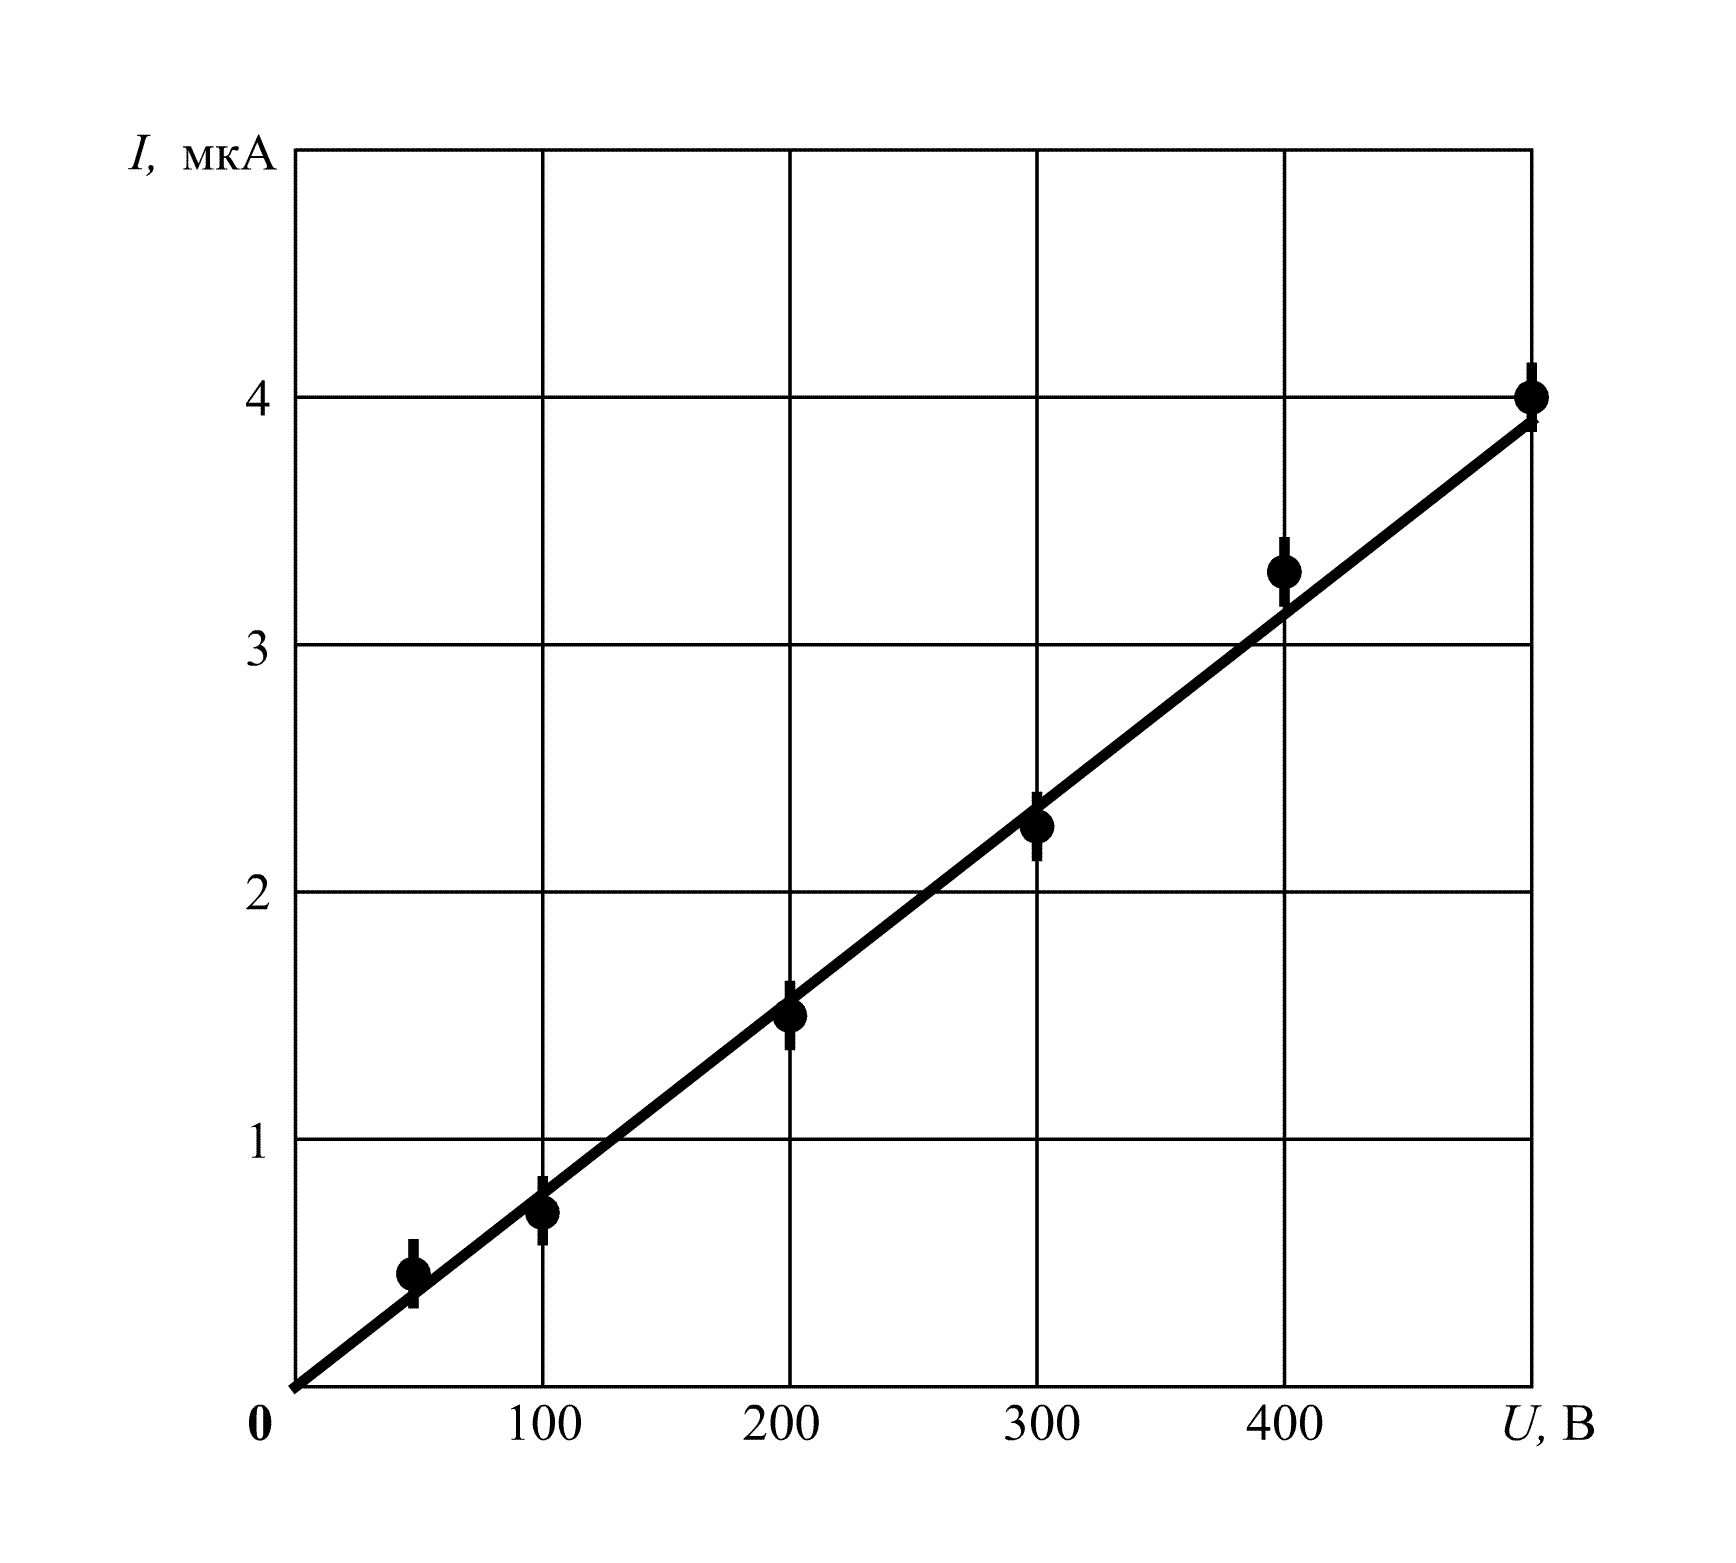
\includegraphics[scale = 0.25, keepaspectratio=true]{Intro-GraphExample.png}
\end{center}
\caption{Вольт-амперная характеристика разрядного тока \label{fig:example-exp-plot}}
\end{figure}


Часто бывает целесообразно построить график зависимости одной измеряемой физической величины (функции) от другой (аргумента). График дает наглядное представление об исследуемой закономерности, поэтому умение правильно строить его "--- необходимое условие для формирования навыка экспериментальной работы. График строят, используя табличную запись результатов.

График необходимо строить на масштабно-координатной (миллиметровой) бумаге в следующей последовательности:

\begin{enumerate}
  \item Установить пределы изменения величин, откладываемых по координатным осям.
  \item  Выбрать масштабы по осям координат в зависимости от погрешности измерений. На миллиметровой бумаге 1~\Units{см} может соответствовать $10^n,\ 2\cdot10^n,\ 5\cdot10^n \ (n = 0, \pm 1, \pm 2, ...)$ единицам физической величины.
  \item Поле графика нужно постараться приблизить к квадрату.
  \item На каждую координатную ось следует наносить шкалу в пределах изменения величин, отложенную в выбранном масштабе, а не координаты точек и не результаты измерений и расчетов.
  \item Буквенные обозначения и единицы физических величин располагаются, как указано на рис.~\ref{fig:example-exp-plot}.
  \item Результаты измерения в виде точек следует наносить на поле графика, не проводя дополнительных линий.
  \item Строить график нужно с помощью лекала или линейки путем осреднения: количество точек над и под графиком должно быть примерно одинаковым. Существуют более строгие способы построения экспериментальных кривых. С ними вы познакомитесь позже.
  \item Погрешности измерения изображаются отрезками в соответствующем масштабе у экспериментальных точек (см.~рис.~\ref{fig:example-exp-plot}) как границы доверительного интервала.
  \item Под графиком помещается название рисунка, пишется номер рисунка и примечания к рисунку.
\end{enumerate}

В таблице~\ref{tab:example-exp} и на рис.~\ref{fig:example-exp-plot} дан пример построения вольт-амперной характеристики несамостоятельного разряда.




\subsection{Содержание протокола лабораторной работы}
% ИЗМ Номер Эн
Лабораторная работа \textnumero N

Наименование работы
\begin{center}
\begin{tabular}{| > {\centering\arraybackslash} m{3cm} | > {\centering\arraybackslash} m{3cm} | > {\centering\arraybackslash} m{3cm}|} \hline
Допуск & Выполнение & Защита \\ \hline
\phantom{Игорь сделал,}& \phantom{выполнил,}& \phantom{защитил на 2их.}\\ \hline
\end{tabular}
\end{center}

\begin{enumerate}
\item Цель работы.
\item Основные теоретические положения и необходимые расчетные
соотношения.
\item Схема установки. Основные данные измерительных приборов.
\item Результаты измерений. Заполнять только ручкой, при обнаружении ошибочного результата аккуратно зачеркнуть его и рядом написать верный результат.
\item Обработка результатов эксперимента. В этом же разделе помещаются графики зависимостей, выполненные на масштабно-координатной (миллиметровой) бумаге. Сравнение полученных данных со справочными данными.
\item Выводы.
\end{enumerate}

\subsection{Порядок работы в физической лаборатории}
К выполнению лабораторной работы следует готовиться заблаговременно (до начала занятий в лаборатории): уяснить цель исследования, методику выполнения измерений, технические приемы измерений. При подготовке к работе нужно ознакомиться с описанием лабораторной работы и, кроме того, проштудировать соответствующие разделы конспекта лекций и учебника.

Протокол лабораторной работы оформляется во время домашней подготовки к работе. Учащиеся, не подготовившие протокол, к выполнению работы не допускаются.

На занятиях лабораторного практикума группа разбивается на бригады по двое учащихся. Протоколы лабораторных работ ведутся каждым учащимся. Учащийся несет персональную ответственность за состояние своего лабораторного журнала.

Перед началом выполнения работы учащиеся должны получить допуск к работе у преподавателя, ведущего занятия. Допуск к работе дается учащимся, знающим основные теоретические и методические особенности выполняемой работы и ознакомившимся с устройством экспериментальной установки. Учащиеся, не получившие допуск к работе в течение первых двадцати минут занятия, к выполнению работы не допускаются. Допуск к работе отмечается преподавателем в протоколе лабораторной  работы с указанием даты.

 Если учащийся не допущен к выполнению работы, то он выполняет работу во время, указанное сотрудниками лаборатории при наличии технической возможности лаборатории. При невыполнении работы в срок ставится неудовлетворительная оценка.

 Если учащийся отсутствует на занятии по уважительной  причине, он должен выполнить работу по дополнительному графику. Обработка результатов измерений  производится во время лабораторных занятий. Получение результата является основанием для отметки о выполнении, которая также ставится преподавателем.

 Последним этапом является защита лабораторной работы, которая производится на специальном зачетном занятии. По указанию преподавателя защита может производиться и на других занятиях. Защита проводится в индивидуальном порядке. Проведение побригадных защит запрещено. В процессе защиты учащийся должен показать знание разделов теории, касающихся вопросов, изучаемых в работе, решить предложенные преподавателем задачи и продемонстрировать хорошее знакомство с особенностями работы на экспериментальной установке. В результате защиты учащийся получает оценку.

\newpage

\setcounter{section}{0}
\setcounter{subsection}{0}
\setcounter{subsubsection}{0}
\setcounter{figure}{0}
\setcounter{table}{0}
\setcounter{equation}{0}
\section*{Вводная лабораторная работа}

{\huge \textbf{Измерения в физическом практикуме}}

\subsection{Измерительные приборы, используемые в практикуме по механике}

Измерительными приборами называют технические устройства, воспринимающие измеряемую величину и выдающие ее значение в виде показания.

Для измерения линейных размеров в лабораторном практикуме применяют линейку, штангенциркуль и микрометр.

% ИЗМ: Я их бессмысленный (на мой взгляд) список заменил на выделение жирным.
% Cначала на параграфы, но, по-моему, они очень уродливые огромные промежутки делают.

\textbf{Линейка.}

Длина измеряется с помощью масштабной линейки.
Величина  наименьшего ее деления называется ценой одного деления.
Обычно цена деления линейки равна 1~\Units{мм}.

\textbf{Штангенциркуль.}

Если длина измеряется с погрешностью до долей миллиметра, то пользуются вспомогательной шкалой измерительного инструмента "--- нониусом. В инструменте, называемом штангенциркулем, используется нониус, имеющий 10~делений, цена деления равна 0,1~\Units{мм}.

Штангенциркуль (рис.~\ref{fig:mzero-caliper}) состоит из миллиметровой линейки~\emph{1}, с одной стороны которой имеется неподвижная ножка~\emph{2}.

Вторая (подвижная) ножка~\emph{3} имеет нониус~\emph{4}. % ИЗМ: "и" - видимо, опечатка, поменяла на точку.
Штангенциркуль может перемещаться вдоль линейки~\emph{1}. Когда ножки~\emph{2}~и~\emph{3} соприкасаются, нуль линейки и нуль нониуса должны совпадать. Для того, чтобы измерить длину предмета~\emph{5}, его помещают между ножками, которые сдвигают до соприкосновения с предметом, и закрепляют винтом~\emph{6}. После этого делают отсчет по линейке и нониусу и вычисляют длину предмета.
% ИЗМ: Убрал "диаметр канавки" - потому что один черт знает, что это такое | все-таки что-то менять по смыслу не стоит
% всякого рода -> разнообразных
Выступающие части ножек~\emph{7}~и~\emph{8} служат для измерения диаметров канавок и разнообразных углублений. На рис.~\ref{fig:mzero-vernier-scale} в увеличенном виде показаны две шкалы штангенциркуля. Сверху изображена шкала масштабной линейки,  снизу "--- шкала нониуса. Определим показания этих шкал.


\begin{figure}[ht]
 \begin{center}
  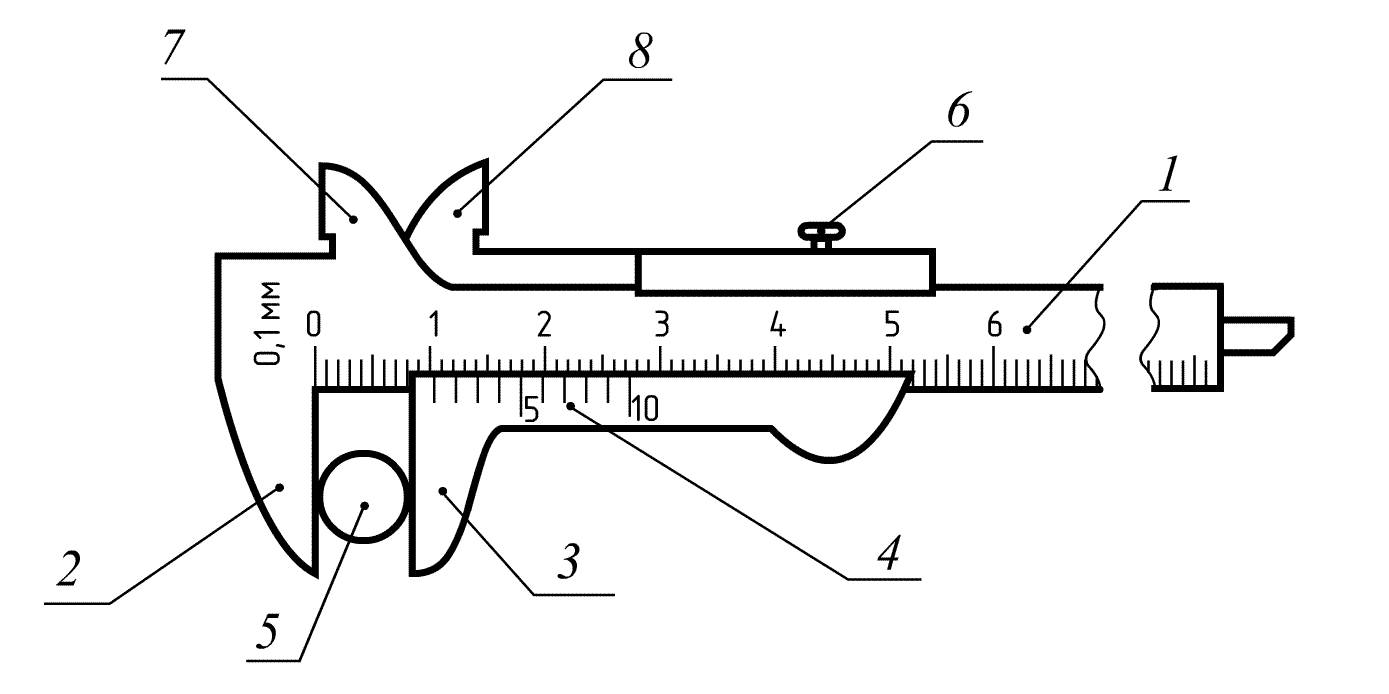
\includegraphics[width = 0.65\textwidth, keepaspectratio=true]{Intro-Caliper}
  \caption{Штангенциркуль \label{fig:mzero-caliper}}
 \end{center}
\end{figure}


\begin{figure}[h]
 \begin{center}
  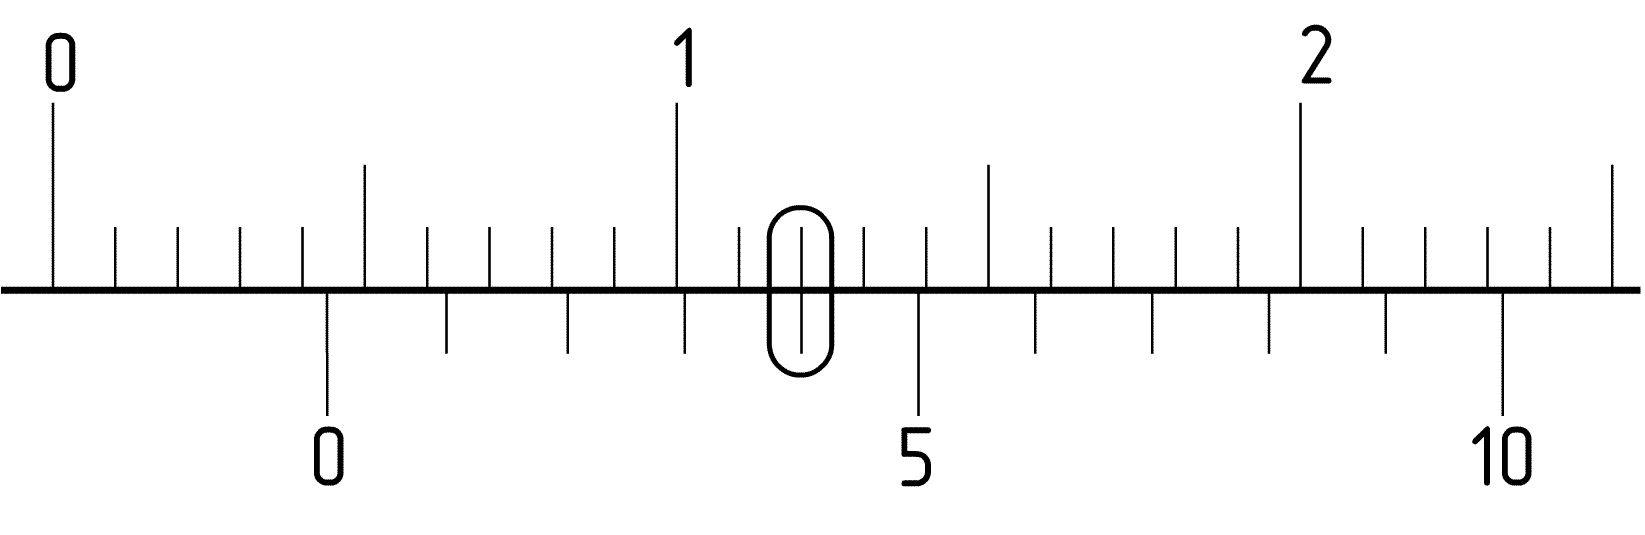
\includegraphics[width = 0.5\textwidth, keepaspectratio=true]{Intro-CaliperVernier}
  \caption{Нониусная шкала \label{fig:mzero-vernier-scale}}
 \end{center}
\end{figure}


%ИЗМ: добавил "измеряемой"
Нуль нониуса находится между 4-м и 5-м делениями масштабной линейки. Это значит, что размер измеряемой детали больше~4 и меньше 5~\Units{мм}. Размер измеряемой детали в миллиметрах можно определить по формуле
\begin{equation}
\label{eq:how-do-i-caliper}
l = k + 0,1\mu
\end{equation}
где $k$ "--- число делений масштабной линейки, укладывающихся в измеряемой длине; \\
$\mu$ "--- число, показывающее тот номер деления нониуса, который совпадает  с некоторым делением шкалы масштабной линейки.

В нашем случае (см.~рис.~\ref{fig:mzero-vernier-scale}) $k = 4$ и $\mu = 4$, так как именно четвертое деление нониуса совпадает с некоторым делением шкалы масштабной линейки (отмечено кружком). Остальные деления нониуса не совпадают с делениями линейки.
% ИЗМ: поставил "и" вместо запятой, добавил "именнно", не выносил k и mu на отдельные строки, они и так отчично выделяются курсивом своим (?) | не, не выделяется

 % Две картинки рядом | У меня не получилось заставить это нормально работать! :(
 % Потом ещё попроубю... Но пока получилось, что подписи сьезжают черте-куда.




\textbf{Микрометр.}

Для измерения с большей точностью (до сотых долей миллиметра) применяют инструмент, называемый микрометром. Микрометр (рис.~\ref{fig:mzero-mu-caliper}) состоит из двух частей: скобы~\emph{1} и микрометрического винта~\emph{2}, который проходит через отверстие скобы~\emph{1} с внутренней резьбой. Против микрометрического винта на скобе имеется упор~\emph{3}. На этом винте закреплен полый цилиндр (барабан)~\emph{4} с делениями по окружности. При вращении микрометрического винта барабан скользит по линейной шкале, нанесенной на стебле~\emph{5}.

\begin{figure}[ht]
 \begin{center}
  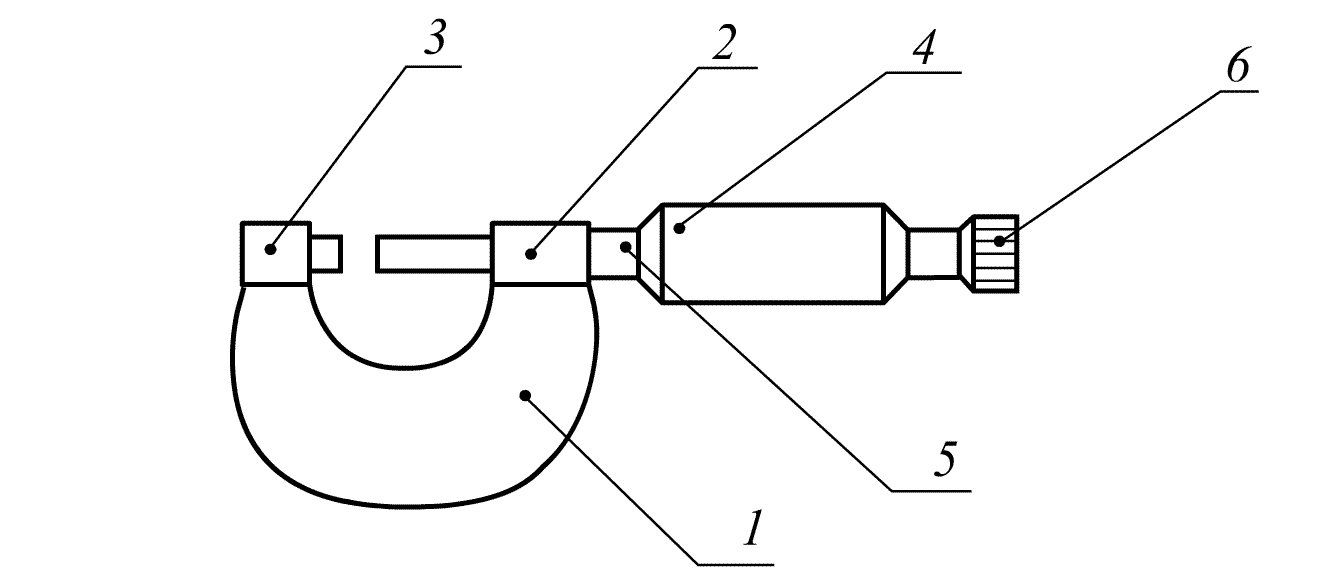
\includegraphics[width = 0.65\textwidth, keepaspectratio=true]{Intro-MuCaliper}
  \caption{Микрометр \label{fig:mzero-mu-caliper}}
 \end{center}
\end{figure}


\begin{figure}[h]
 \begin{center}
  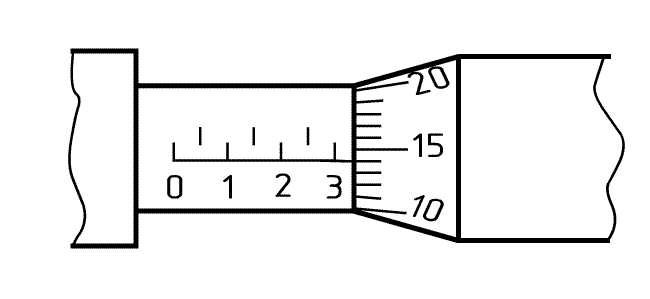
\includegraphics[width = 0.5\textwidth, keepaspectratio=true]{Intro-MuCaliperVernier}
  \caption{Нониусная шкала микрометра\label{fig:mzero-mu-caliper-vernier}}
 \end{center}
\end{figure}

Во время измерения предмет помещают между упором~\emph{3} и винтом~\emph{2} и вращают винт до тех пор, пока измеряемый предмет не будет зажат между упором~\emph{3} и концом винта~\emph{2}.

Измеряемая деталь должна зажиматься микрометром с определенным усилием, дозволенным техническими нормами эксплуатации. С этой целью при зажиме детали необходимо вращать не барабан~\emph{4}, а головку~\emph{6}, называемую трещоткой. В тот момент, когда сжимающее усилие достигнет  нормы, дальнейшее вращение головки будет сопровождаться звуком трещотки,  означающим, что микрометрический винт больше не вращается. В это время шкалы микрометра показывают размер детали.

В данной работе применяется микрометр, у которого цена деления линейной шкалы стебля равна 0,5~\Units{мм}. Верхние и нижние риски шкалы сдвинуты относительно друг друга на полмиллиметра (см. рис.~\ref{fig:mzero-mu-caliper-vernier}), цифры проставлены только для делений нижней шкалы, т.~е. нижняя шкала "--- обычная миллиметровая. Если барабан сделает один оборот, он переместится вдоль оси стебля на одно деление, т.~е. на 0,5~\Units{мм}. Число делений барабана равно~50. Следовательно, цена деления барабана равна 0,01~\Units{мм}.




\subsection{Определение плотности твердых тел}

Целью эксперимента является определение плотностей тел правильной геометрической формы (металлических цилиндров) по результатам измерения масс~$m_1$ и~$m_2$, диаметров~$d_1$ и~$d_2$, высот~$h_1$ и~$h_2$, пользуясь формулой
\begin{equation}
\label{fig:mzero-density}
\rho = \frac{m}{V} = \frac{4m}{\pi d^2 h}.
\end{equation}

Массы определяют путем взвешивания на технических весах. Диаметры и высоты цилиндров находят с помощью штангенциркуля. В заключение необходимо обработать полученные данные и вычислить погрешности измерений.

\subsection{Порядок выполнения работы}

\begin{enumerate}
\item Произвести однократное взвешивание каждого цилиндра на технических  весах. Записать массу в граммах в таблицу~\ref{tab:mzero-params-table} с указанием погрешности  измерений (инструментальной). Инструкции по проведению взвешивания получите у преподавателя и дежурного инженера лаборатории. % "массу в граммах" не сходится с таблицей: там кг
\item Произвести пять измерений диаметров и высот каждого цилиндра.


\end{enumerate}
% странно тут без гор. линий, кажется гор. линии нужны где номер (почему они не сделали №? хотя так даже красивее) измерения, где d и h
\begin{table}[h]
% Глаза мои!
\caption{\label{tab:mzero-params-table}}
\begin{center}
\begin{tabular}{|>{\centering\arraybackslash} m{2cm}|>{\centering\arraybackslash} m{2cm}|>{\centering\arraybackslash} m{1.3cm}|>{\centering\arraybackslash} m{1.3cm}|>{\centering\arraybackslash} m{1.3cm}|>{\centering\arraybackslash} m{1.3cm}|>{\centering\arraybackslash} m{1.3cm}|>{\centering\arraybackslash} m{1.3cm}|>{\centering\arraybackslash} m{1.3cm}|}
\hline
Номер цилиндра & Номер измерения & $d$,~\Units{мм} & $\Delta d$,~\Units{мм} & $h$,~\Units{мм} & $\Delta h$,~\Units{мм} & $m$,~\Units{кг} & $\Delta m$,~\Units{кг} & $\rho$,~\Units{$\text{кг}/\text{м}^3$} \\ \hline
\multirow{5}*{\Huge 1} & 1 & & & & & & & \\
 & 2 & & & & & & & \\
 & 3 & & & & & & & \\
 & 4 & & & & & & & \\
 & 5 & & & & & & & \\ \hline
\multirow{5}*{\Huge 2} & 1 & & & & & & & \\
 & 2 & & & & & & & \\
 & 3 & & & & & & & \\
 & 4 & & & & & & & \\
 & 5 & & & & & & & \\ \hline
\end{tabular}
\end{center}
\end{table}

\subsection{Обработка результатов измерений}
% мб сделать multirow в шапке, чтобы 1. степень нормально была, 2. похоже было на предыдущую
\begin{table}[h!]
% Глаза мои!
\caption{\label{tab:mzero-processing-table}}
\begin{center}
\begin{tabular}{|>{\centering\arraybackslash} m{0.2245\linewidth}|>{\centering\arraybackslash} m{0.2245\linewidth}|>{\centering\arraybackslash} m{0.2245\linewidth}|>{\centering\arraybackslash} m{0.2245\linewidth}|}
\hline
Номер измерения & $x_i$ & $\MTDMean{x} - x_i$ & $\left(\ \MTDMean{x} - x_i\right)^2$ \\ \hline
1 & & & \\ \hline
2 & & & \\ \hline
3 & & & \\ \hline
4 & & & \\ \hline
5 & & & \\ \hline
$\MTDMean{x}$ & & \multicolumn{2}{c|}{$\isum \left(\ \MTDMean{x} - x_i\right)^2 = \phantom{295 \text{баллов по ЕГЭ}}$} \\ \hline
% Фантомы - чтобы оно налево съезжало
\end{tabular}
\end{center}
\end{table}
% ИЗМ: "равно" внизу поставил, оно там явно нужно.

\begin{enumerate}
\item Определение плотности тел предложенным методом представляет собой косвенное измерение. Как следует из теории погрешностей, необходимо определить погрешности прямых измерений, т.~е. $\Delta h$, $\Delta d$, $\Delta m$.

\item Для каждой из величин $m$, $h$ и $d$ составляют таблицы по образцу таблицы~\ref{tab:mzero-processing-table}. %зачем таблица для массы? вроде как мы измеряем $m$ 1 раз, а потом нас инженер оттуда выгоняет, а погрешность мы записываем туда инструментальную.

\item Далее проводятся соответствующие расчеты:
\[
    \Delta h = 2,8 \sqrt{\frac{\isum\left(\ \MTDMean{h} - h_i \right)^2}{5 \cdot 4}},
\]
\[
    \Delta d = 2,8 \sqrt{\frac{\isum\left(\ \MTDMean{d} - d_i \right)^2}{5 \cdot 4}}.
\]
Среднее значение плотности
\[
\MTDMean{\rho} = \frac{4\MTDMean{m}}{\pi \MTDMean{d}^2 \MTDMean{h}}.
\]
\item Окончательный результат должен быть представлен в виде
\[
\rho =\ \MTDMean{\rho} \pm \Delta \rho.
\]

В данной работе рекомендуется рассчитывать по соотношению %мб "В данной работе \Delta \rho рекомендуется"
\[
\Delta \rho = \MTDMean{\rho} \sqrt{\left(\frac{\Delta m}{\MTDMean{m}}\right)^2 + \left(2\frac{\Delta d}{\MTDMean{d}}\right)^2 + \left(\frac{\Delta h}{\MTDMean{h}}\right)^2}.
\]

\item Ориентируясь на внешние признаки материалов цилиндров, сравнить полученные результаты с табличными значениями плотностей материалов. Результаты всех измерений и расчетов должны быть представлены в системе единиц СИ.
\end{enumerate}

\subsection{Контрольные вопросы}
\begin{enumerate}
% ИЗМ: Закавычил
\item Что значит <<измерить физическую величину>>?
\item Какие погрешности называются систематическими, какие "--- случайными?
\item Какие измерения называются прямыми, какие "--- косвенными? Приведите примеры прямых и косвенных измерений,  проведенных в данной работе.
    % ИЗМ: "а какие?" Кажется, немного менее неуклюже{
\item Какие погрешности называются абсолютными, а какие "--- относительными?
\item Каким образом в данной работе проводилась обработка результатов измерений?
\end{enumerate}

\end{document}

